% Technical document. Build: cd submission && ./build.sh  (or latexmk -pdf technical.tex)
\documentclass[10pt,a4paper,twocolumn]{article}

\providecommand{\teamname}{TikiData}
\providecommand{\members}{Huyen Trang Ngo, Hoang Phuc Ngo, Thanh Long Ly, Khanh Duong Pham, Duc Anh Pham}

\usepackage[T1]{fontenc}
\usepackage[utf8]{inputenc}
\usepackage{lmodern}
\usepackage[margin=1.6cm,columnsep=0.6cm]{geometry}
\usepackage{amsmath,amssymb}
\usepackage{graphicx}
\usepackage{booktabs}
\usepackage{enumitem}
\usepackage{xcolor}
\usepackage{caption}
\usepackage{listings}
\usepackage{titlesec}
\usepackage{tabularx}
\usepackage{flushend}
\usepackage[hidelinks]{hyperref}
\titlespacing*{\section}{0pt}{1.1ex plus .3ex}{0.6ex}
\titlespacing*{\subsection}{0pt}{0.9ex plus .2ex}{0.4ex}
\titlespacing*{\paragraph}{0pt}{0.6ex plus .2ex}{0.6em}
\titleformat*{\section}{\large\bfseries}
\titleformat*{\subsection}{\normalsize\bfseries}
\setlength{\textfloatsep}{8pt plus 2pt}
\setlength{\floatsep}{6pt plus 2pt}
\setlength{\dbltextfloatsep}{8pt plus 2pt}
\setlength{\abovecaptionskip}{3pt}

\setlist{itemsep=0pt,topsep=2pt,parsep=0pt,leftmargin=1.2em}
\captionsetup{font=small,labelfont=bf}
\lstset{basicstyle=\ttfamily\scriptsize,columns=fullflexible,frame=single,backgroundcolor=\color{gray!6},
        breaklines=true,keepspaces=true}
\newcommand{\spellF}{\texttt{spellF1}}
\newcommand{\macroF}{\texttt{macroF1}}

\title{\bfseries Learning Ball Possession from Clean Tracking for Noisy Automatic Tracking:\\
a Switch-Gated Possession Model}
\author{\textbf{\teamname}\\ \members\\[2pt]
\small More than a Hack 2027, Phase 1\\
\small \url{https://github.com/tlong-ds/tikidata-possession}}
\date{}

\begin{document}
\maketitle

\begin{abstract}
Our model learns possession from labelled DFL and Metrica matches and transfers to the target's
noisy automatic tracking. We measure the target tracking's failure statistics and corrupt the
clean training tracking to match them. A team-pooled set encoder and a
bidirectional GRU predict per-frame H/A/D and a \emph{change-of-possession} signal, helped by explicit
features of the contest around the ball and of sudden changes in ball motion. A four-state Viterbi
decoder uses the change signal to price team changes and is tuned for \spellF. Before final
retraining, the selected configuration scores mean \spellF{} 0.671 and mean \macroF{} 0.906 across
five fixed degraded versions of the Bundesliga match J03WN1. The submission model is retrained
once with the development match added.
\end{abstract}

% ------------------------------------------------------------------------------------------------
\section{Approach}\label{sec:approach}

\begin{figure*}[t]
  \centering
  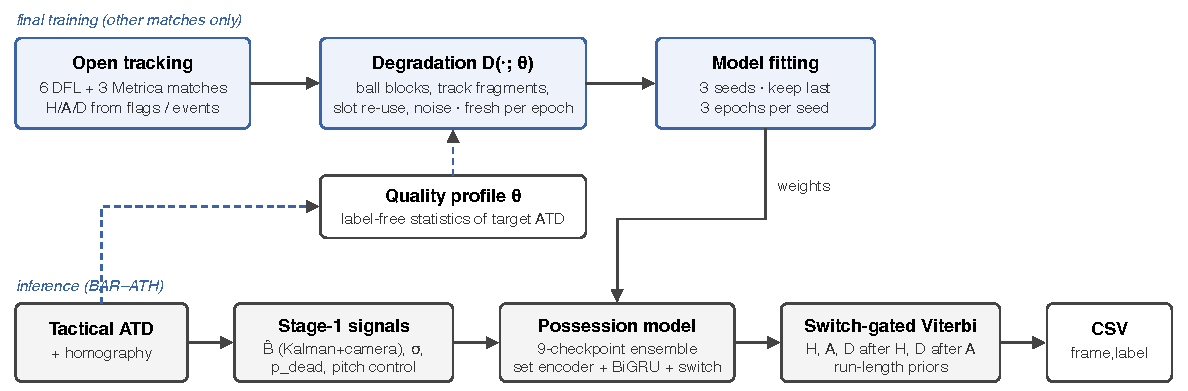
\includegraphics[width=0.92\textwidth]{figures/pipeline.pdf}
  \caption{Training uses only other matches (DFL and Metrica, \S\ref{sec:data}), corrupted to
  match a label-free quality profile $\theta$ of the target tracking. At inference, stage-1 signals,
  a 9-checkpoint ensemble and the decoder run on the target.}
  \label{fig:pipeline}
\end{figure*}

We transfer possession knowledge from labelled matches with clean tracking to the target's
automatic tracking, in which the ball is unseen on 41\% of graded frames and
player tracks fragment. The pipeline (Figure~\ref{fig:pipeline}) has four parts:
\begin{enumerate}
  \item \textbf{Label-free degradation} (\S\ref{sec:degrade}): measure the target tracking's failure
        statistics and corrupt the clean training tracking the same way.
  \item \textbf{Stage-1 signals} (\S\ref{sec:degrade}): a filtered ball estimate with uncertainty, a
        dead-ball probability and pitch control, computed before the network.
  \item \textbf{A switch-gated sequence model} (\S\ref{sec:model}--\ref{sec:inputs}): a team-pooled
        set encoder and BiGRU with a change-of-possession head, plus explicit contest and
        ball-touch features.
  \item \textbf{A switch-gated Viterbi decoder} (\S\ref{sec:model}): turns frame posteriors into
        possessions, pricing team changes with the switch head.
\end{enumerate}

\paragraph{Why this design.}
\begin{itemize}
  \item \emph{The ball is often missing}, so the model reads possession cues from player motion.
        We fit the degradation of the training tracking to the target's measured failure statistics.
  \item \emph{Proximity and pitch control provide complementary cues}: the nearest team is right
        on 67\% of live development frames, so the network combines distances and pitch control
        with player motion.
  \item \emph{The metric counts possessions}: a model right on most frames still ranks poorly if it
        splits or merges possessions, so changes are predicted explicitly and the decoder is tuned
        for \spellF.
\end{itemize}

% ------------------------------------------------------------------------------------------------
\section{Training data}\label{sec:data}

\paragraph{DFL/Sportec open data~\cite{bassek2025}.} Bundesliga matches with 25\,Hz corrected
tracking (CC BY 4.0) whose per-frame \texttt{BallStatus} and \texttt{BallPossession}
flags, set by the data provider, have exactly the semantics of the target ground truth; used as
given. The split was fixed before modelling: five training matches and one
development match (J03WN1).

Ten fixed versions of the full J03WN1 match are generated with distinct tracking-degradation
seeds (\S\ref{sec:degrade}). Five are used to choose features, checkpoints and decoder parameters;
the remaining five evaluate the fixed configuration. All share the same match and possession labels.

\paragraph{Metrica sample data~\cite{metrica}.} Three anonymised public matches from another league,
used for training only. Per-frame H/A/D labels are derived from the events by fixed rules (dead from a
ball-out or whistle event to the restart, otherwise the team of the last controlling event), the
ball is mapped to the DFL convention, and the matches are degraded like the DFL ones. Downloads
are pinned to a source commit and verified by SHA-256.

\paragraph{Final model.} After configuration selection, we retrain with J03WN1 added
(six Bundesliga and three Metrica matches). We average epochs 8, 9 and 10 of seeds 1, 2 and 3,
keeping the decoder settings fixed from selection.

\paragraph{Reproduction.} Linux, Python 3.12.11. Set the bundle path below and run from the
repository root. The CSV is validated and compared across two CPU thread counts.
\begin{lstlisting}[aboveskip=3pt,belowskip=3pt]
pip install numpy==2.5.4 scipy==1.18.1 \
  pandas==3.1.1 torch==2.15.0
export MTAH_DATA_DIR=/path/to/provided-data
python -m src.submit run --model final_metrica \
  --check-twice --out TikiData.csv
sha256sum TikiData.csv
\end{lstlisting}
Expected SHA-256:\\
{\scriptsize\texttt{aca26c78203fdd4ecf233a89754ec4dd2c3bb4db9373625279e85bcc582b59fd}}

The target tracking supplies the noise profile (\S\ref{sec:degrade}) and the ball-touch lag
(\S\ref{sec:inputs}).

% ------------------------------------------------------------------------------------------------
\section{Method}

\subsection{Label-free target profiling and degradation}\label{sec:degrade}

From the target ATD, we compute a quality profile $\theta$:
\begin{itemize}
  \item ball-visible share, overall and before restarts;
  \item run lengths of missing and visible ball;
  \item ball visibility by crowd size and pitch region;
  \item per-team player counts and their autocorrelation at 1/5/30\,s;
  \item slot occupancy, absence runs and churn;
  \item missingness and roughness of speeds.
\end{itemize}
A degradation operator $D(\cdot;\theta)$ corrupts a clean DFL half with restart-aware ball dropout
in blocks, player-track fragmentation with slot re-use, position noise and missing speeds. Its
strengths are calibrated on one training match so that the statistics of $D(\text{clean})$ match
$\theta$. A new realisation is drawn every epoch: domain randomisation~\cite{tobin2017} fitted
to measured target statistics.

\paragraph{Stage-1 signals.} Three hand-built signals, fitted on DFL training matches only, are
computed before the network and used as its inputs:
\begin{itemize}
  \item \textbf{Ball estimate $\hat B$ with uncertainty $\sigma$.} A two-way Kalman/RTS
        smoother~\cite{rauch1965} with a Mahalanobis gate, which separates touches (velocity reset)
        from spurious detections (rejected). Over long gaps, $\hat B$ is fused with the camera
        centre projected through the homography, because the tactical camera follows play.
  \item \textbf{Dead-ball probability.} A logistic model of ball speed, crowding near the ball,
        distance to the nearest player, mean player speed and a soft out-of-bounds term.
  \item \textbf{Pitch control~\cite{spearman2018,fernandez2018} at $\hat B$.} Shrunk towards 0.5 as
        $\sigma$ grows.
\end{itemize}

\subsection{Switch-Gated Possession Model}\label{sec:model}

\begin{figure*}[t]
  \centering
  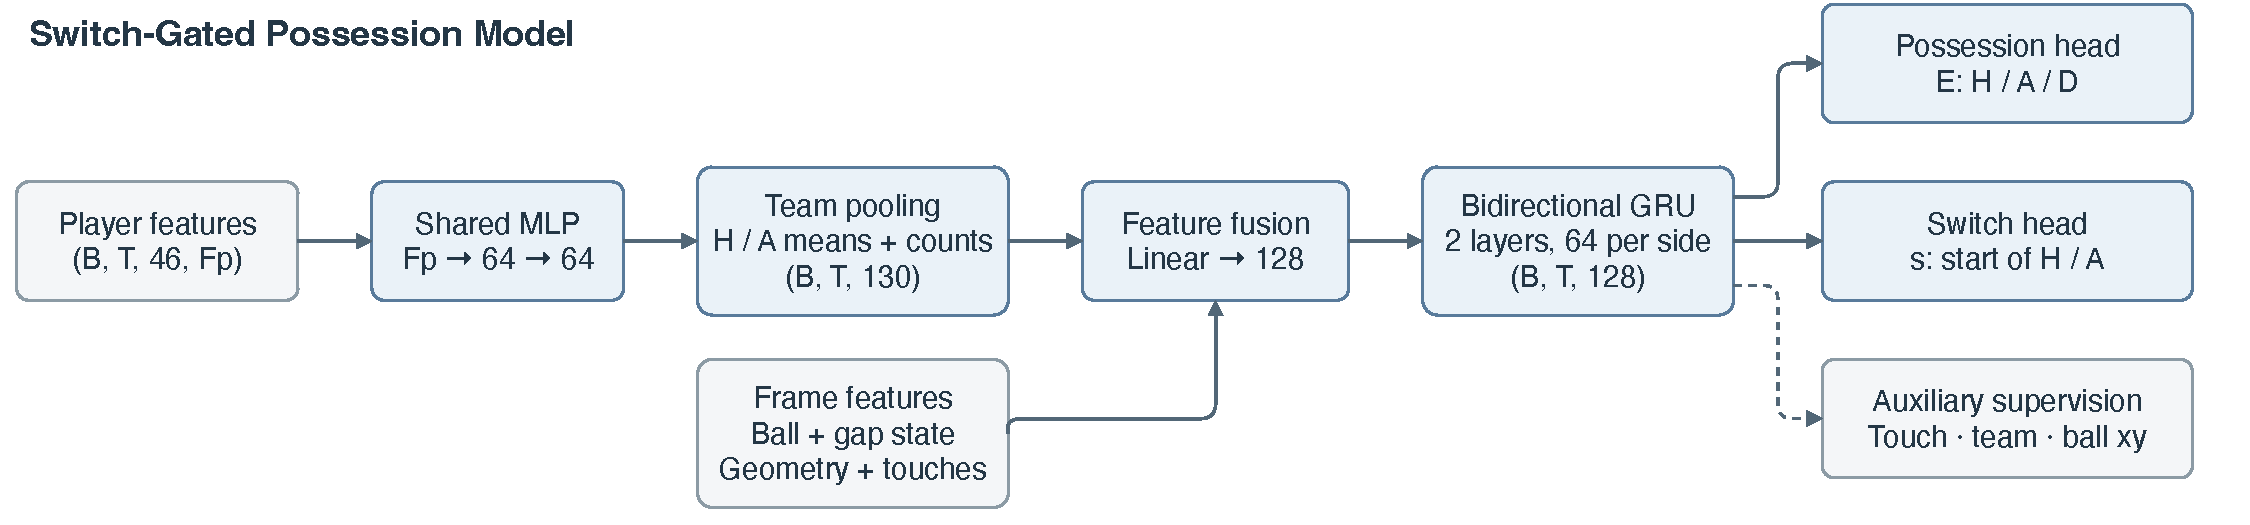
\includegraphics[width=\textwidth]{figures/architecture.pdf}
  \caption{Single-checkpoint architecture. A shared player encoder and team pooling feed a BiGRU
  with possession and switch heads. B is batch size, T is sequence length and Fp is the
  player-feature dimension.}
  \label{fig:architecture}
\end{figure*}

The shared player MLP has two 64-unit layers. Masked team mean-pooling (Deep
Sets~\cite{zaheer2017}) uses team membership and includes player counts, making the representation
invariant to within-team slot reassignment. The pooled vectors and frame features are projected
to 128 dimensions, then passed through a 2-layer bidirectional GRU with 64 units per direction.
Its switch head predicts the start of an H or A possession, including restarts
(Figure~\ref{fig:architecture}).

\paragraph{Training.}
\begin{itemize}
  \item \emph{Losses:} cross-entropy on H/A/D, with label smoothing near changes and an extra term
        within $\pm1$\,s of a change (weight 0.5); BCE on switch and touch; Huber on ball position.
  \item \emph{Augmentation:} team swap (with the $x$-axis mirrored) and a vertical flip.
  \item \emph{Windows:} 128 steps at stride 2 ($\approx$10\,s).
  \item \emph{Initialisation:} new input columns start at zero, preserving the initial network
        outputs. Configuration training uses a 3-epoch adaptation phase followed by 7 epochs
        with all weights unfrozen.
  \item \emph{Checkpoint choice:} for each of 3 seeds we keep the 3 epochs with the best \spellF{}
        on the development match, measured \emph{through the decoder}. The 9 checkpoints are averaged.
\end{itemize}

\paragraph{Decoder.} Viterbi~\cite{rabiner1989} over $\{\mathrm H,\mathrm A,\mathrm D_{\mathrm H},\mathrm
D_{\mathrm A}\}$; splitting D by the last owner lets a stoppage remember who had the ball.
Emissions are the posteriors $E_t$ scaled by $\lambda$.
\begin{itemize}
  \item \emph{Live $\to$ D:} hazard $\mathit{share}_{\text{dead}}/(L_{\text{alive}}\cdot
        \text{fps})$. D runs have expected length $L_{\text{dead}}$. Both are learned on DFL:
        $L_{\text{alive}} = 7.29$\,s, $L_{\text{dead}} = 24.5$\,s.
  \item \emph{H $\to$ A:} probability $\operatorname{clip}(c\cdot\hat s_t^{\mathrm A},\,
        p_{\min},\, p_{\max})$, where $\hat s$ is the switch head max-pooled over $\pm w$ frames;
        A $\to$ H is symmetric.
  \item \emph{Leaving D for team $j$:} a restart prior, $P(\text{other team}) = 0.693$, gated by
        $s_t^{j}$.
\end{itemize}
All decoder parameters are grid-searched on the development match for \spellF. The submitted model uses
$c = 0.02$, $\lambda = 0.5$ and $w = 3$.

\subsection{Model inputs}\label{sec:inputs}

\paragraph{Base channels.}
\begin{itemize}
  \item \emph{Per player:} position, velocity, team, presence, offset and distance to $\hat B$, and
        how long the track has existed and will continue to exist.
  \item \emph{Per frame:}
  \begin{itemize}
    \item $\hat B$, $\sigma$ and its source;
    \item camera centre and pan;
    \item time since and until the ball is seen;
    \item for each team, how many players have just vanished or will soon reappear (a crowd
          vanishing from tracking marks a duel);
    \item the stage-1 dead-ball and pitch-control probabilities.
  \end{itemize}
\end{itemize}

\paragraph{Contest geometry.} Explicit distance features complement team mean pooling.
\begin{itemize}
  \item \emph{Per team:} the closeness $\exp(-d/5\,\mathrm m)$ of its nearest and second-nearest
        player to $\hat B$, the number of players within 5\,m, and the change of its nearest
        distance over the past and next 0.4\,s. These are set to zero when the team's player count
        or $\hat B$'s source changes, guarding against movement artefacts at track gaps.
  \item \emph{Per player:} closeness to $\hat B$, closeness to the nearest opponent, and approach
        speed towards $\hat B$.
\end{itemize}

\paragraph{Ball touch.} Many missed possessions are a single short touch by the other team between
two possessions of the same team (an intercepted pass that bounces back). The Kalman estimate
smooths such touches away, so we measure them on the \emph{observed} ball. With incoming and
outgoing velocities over a lag $L$, we compute:
\begin{itemize}
  \item the kick strength $\lvert v_{\text{out}} - v_{\text{in}}\rvert$, the turn cosine and both
        speeds;
  \item for each team, kick $\times \exp(-d/1.5\,\mathrm m)$ to the team's nearest player,
        max-pooled over $\pm0.4$\,s.
\end{itemize}

\paragraph{Choosing the ball-motion lag.} The target ball is smoothed: it repeats its previous
coordinate on 0.08\% of visible frames, against 48.8\% for the DFL ball, and its turns spread over
about 0.4\,s. With $L = 0.2$\,s, kick peaks occur 4.8 times per minute of visible ball on the
target, against 24.3 on the development match. With $L = 0.4$\,s the rates match (19.4 against
21.5), so the submitted model uses $L = 0.4$\,s. This is a label-free statistic of the target, in
the same spirit as \S\ref{sec:degrade}.

\paragraph{Development ball smoothing.} For target-like sensitivity checks, the visible
development ball is smoothed with a Gaussian of 0.24\,s plus 0.4\,m of coloured noise. Player
tracking and possession labels are unchanged.

% ------------------------------------------------------------------------------------------------
\section{Results}

\subsection{Evaluation protocol and metrics}\label{sec:evaluation}

The comparison uses the full Bundesliga match J03WN1, kept separate from training during
configuration evaluation. Features, checkpoints and decoder parameters are fixed before scoring
five tracking-degradation versions generated with random seeds distinct from those used for
tuning (\S\ref{sec:data}). All systems are scored on the same five versions, with the same
possession labels and evaluator. All reported experiments were tested on Linux.

H and A denote home- and away-team possession; D denotes a dead ball. We report two metrics.

\paragraph{\spellF{}: possession intervals.} A possession interval is a maximal run of H or A,
with the halves kept separate. Predicted and reference intervals of the same team are matched
one-to-one, greedily in decreasing temporal intersection-over-union (IoU). An interval-level F1
is computed at each IoU threshold in $\{0.3,0.4,0.5,0.6,0.7\}$; \spellF{} is the mean of these
five values.

\paragraph{\macroF{}: frame labels.} F1 is computed separately for H, A and D over graded
frames; \macroF{} is the unweighted mean of the three class scores. Ground-truth X frames are
excluded from this calculation, and a predicted X on a graded frame counts as a miss.

\paragraph{Aggregation.} For each metric, we report the mean and sample standard deviation of
five separately scored versions. These summaries quantify tracking-degradation variability
within J03WN1.

\subsection{Training data and optimisation}

For the evaluated configuration, five DFL and three Metrica matches provide 1,139,396 labelled
frames at 25\,Hz, or 12.66\,hours: 7.94\,hours from DFL and 4.72\,hours from Metrica. Each original
frame is counted once, before generating tracking corruptions. The H/A/D proportions are
29.7\%, 28.1\% and 42.2\%, respectively. This class imbalance makes the separate class
contributions to \macroF{} useful when interpreting frame classification.

The nine retained checkpoints come from epochs 8/9/10, 7/8/10 and 8/9/10 for seeds 1, 2 and 3, respectively.
They all follow the initial three-epoch adaptation phase. Their predicted probabilities are
averaged before decoding.

\begin{figure*}[t]
  \centering
  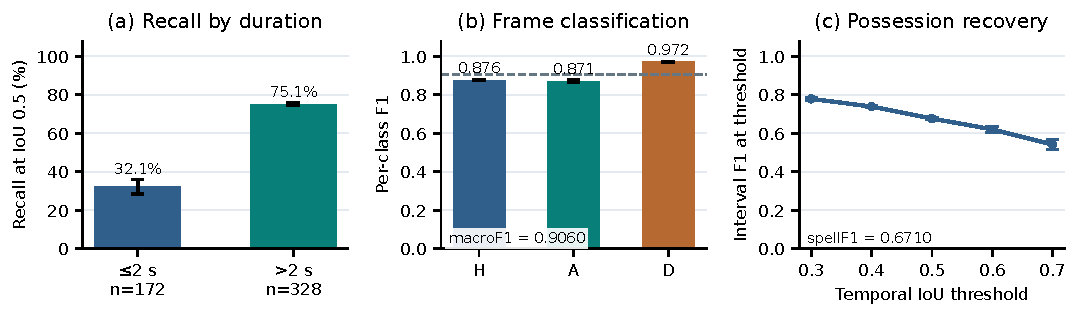
\includegraphics[width=\textwidth]{figures/training_analysis.pdf}
  \caption{Analysis of the evaluated configuration. (a) Recall at IoU 0.5 for true possessions
  lasting at most 2\,s ($n=172$) and longer ones ($n=328$). (b) H/A/D class F1 scores whose unweighted
  mean is \macroF. (c) Possession-interval F1 at each IoU threshold, whose mean is \spellF.
  All panels use the same five evaluation versions as Table~\ref{tab:main}; error bars are
  sample standard deviations across those versions.}
  \label{fig:analysis}
\end{figure*}

\subsection{Main results}

\noindent\begin{minipage}{\columnwidth}
Table~\ref{tab:main} compares the Switch-Gated Possession Model with the nearest-player +
50-frame vote baseline on J03WN1. Both metrics are higher for the model on all five versions.

{\centering\small\setlength{\tabcolsep}{4pt}
  \begin{tabular}{@{}lcc@{}}
    \toprule
    system & \spellF{} & \macroF{} \\
    \midrule
    Nearest-player & 0.2125 $\pm$ 0.0105 & 0.4746 $\pm$ 0.0093 \\
    \textbf{Switch-Gated} & \textbf{0.6710 $\pm$ 0.0102} & \textbf{0.9060 $\pm$ 0.0028} \\
    \bottomrule
  \end{tabular}
  \captionof{table}{Mean $\pm$ s.d.\ over five fixed degraded versions of J03WN1, held out from
  training. The model uses DFL + Metrica. Results precede final retraining.}
  \label{tab:main}
\par}
\end{minipage}

The absolute gains over the baseline are $0.4585$ in \spellF{} and $0.4315$ in \macroF.
Across versions, the model's \spellF{} ranges from 0.6611 to 0.6827 and its \macroF{} from
0.9027 to 0.9092. The small spread measures stability to the sampled tracking corruptions within
this match. The submitted ensemble is subsequently retrained with J03WN1 added, following
\S\ref{sec:data}.

\subsection{What the trained model gets wrong}

All diagnostics below use the evaluated model and the same five versions as Table~\ref{tab:main}.
The mean class F1 scores are 0.8757 for H, 0.8706 for A and 0.9718 for D
(Figure~\ref{fig:analysis}b). Their mean gives \macroF{} 0.9060. The high D score raises this
average, while both live-team class scores remain below 0.88.

\paragraph{Possession recovery.} Interval F1 falls from 0.7787 at IoU 0.3 to 0.5416 at IoU 0.7
(Figure~\ref{fig:analysis}c), showing sensitivity to temporal overlap requirements. The model
predicts 391.2 possessions on average against 500 true, 21.8\% fewer. Of the 500 true possessions,
172 last at most 2\,s. At IoU 0.5, mean recall is 32.1\% for these short possessions and 75.1\%
for longer ones (Figure~\ref{fig:analysis}a). The high \macroF{} therefore coexists with missed
short possession intervals.

\paragraph{Changes and visibility.} On truly live H/A frames, the fraction labelled with the
correct team is 74.3\% within $\pm1$\,s of a true team change and 91.0\% elsewhere; predicting D
on such a frame counts as wrong. This neighbourhood covers 27.8\% of live frames and contains
64.3\% of direct H/A misclassification errors. The same correct-team fraction is 90.3\% when
the ball is visible and 78.7\% when unseen. These errors concentrate where brief team changes
and missing ball observations make the possession boundary hardest to recover.

% ------------------------------------------------------------------------------------------------
\section{Limitations}

\begin{itemize}
  \item \textbf{Evaluation coverage.} Selection and evaluation share J03WN1's events and labels,
        using distinct tracking-degradation seeds. Reported variability concerns tracking errors
        within one match; generalisation across matches remains open.
  \item \textbf{Source--target transfer.} Transfer depends on how well the fitted corruptions
        represent the target's ball motion, missing observations and player-track fragmentation.
  \item \textbf{Long ball gaps.} Reconstruction relies on camera motion and player context;
        plausible ball locations can support different possession assignments.
\end{itemize}

% ------------------------------------------------------------------------------------------------
\begin{thebibliography}{8}\footnotesize\setlength{\itemsep}{0pt}
\bibitem{bassek2025} M.~Bassek et al. An integrated dataset of spatiotemporal and event data in
  elite soccer. \emph{Scientific Data}, 2025. doi:10.1038/s41597-025-04505-y.
\bibitem{spearman2018} W.~Spearman. Beyond expected goals. \emph{MIT Sloan SAC}, 2018.
\bibitem{fernandez2018} J.~Fern\'andez, L.~Bornn. Wide open spaces. \emph{MIT Sloan SAC}, 2018.
\bibitem{zaheer2017} M.~Zaheer et al. Deep sets. \emph{NeurIPS}, 2017.
\bibitem{tobin2017} J.~Tobin et al. Domain randomization for transferring deep neural networks from
  simulation to the real world. \emph{IROS}, 2017.
\bibitem{rabiner1989} L.~Rabiner. A tutorial on hidden Markov models. \emph{Proc.\ IEEE}, 1989.
\bibitem{rauch1965} H.~Rauch, F.~Tung, C.~Striebel. Maximum likelihood estimates of linear dynamic
  systems. \emph{AIAA J.}, 1965.
\bibitem{metrica} Metrica Sports. Sample data.
  \url{https://github.com/metrica-sports/sample-data} (commit e706dd5).
\end{thebibliography}

% ------------------------------------------------------------------------------------------------
\appendix
\section{Assets and possession rules}

\paragraph{Missing and noisy tracking.} Target-matched degradation, an uncertainty-aware
Kalman/RTS ball estimate and explicit gap features address tracking failures at training and
inference (\S\ref{sec:degrade}--\ref{sec:inputs}).

\paragraph{Provided assets.}
\begin{itemize}
  \item \emph{Tactical ATD:} main input, and the source of $\theta$, the touch lag and the
        smoothing check.
  \item \emph{Homography:} camera centre.
  \item \emph{EPTS metadata:} attack direction per half.
  \item \emph{Smart Tagging} (Metrica's automatic tagging): the start times of \texttt{SET PIECES}
        tags as label-free restart anchors for $\theta$ (ball visibility before restarts,
        \S\ref{sec:degrade}), and the two \texttt{Kick Off (Start)} tags to place each half's kickoff
        (possession rules below).
  \item \emph{Public 5-minute ground truth:} end-to-end pipeline check.
\end{itemize}

\paragraph{Possession rules.} The model learns the provider's convention from DFL labels, which
matches the challenge's definition. The decoder adds
run-length priors on top.
\begin{itemize}
  \item \emph{Loose balls:} possession stays with the last owner until the other team controls the
        ball; the decoder prices a team change through the switch head, so a loose phase without a
        switch signal keeps the previous team.
  \item \emph{Challenges and deflections:} ownership stays with the previous team through
        deflections and aerial duels until the other team gains control. The ball-touch features
        supply touch evidence; the switch head learns possession changes from the DFL labels.
  \item \emph{Restarts:} every stoppage is D. The D state remembers the last owner
        ($\mathrm D_{\mathrm H}$/$\mathrm D_{\mathrm A}$); leaving it, the ball goes to the other
        team with prior 0.693 (learned on DFL), overridden by the switch head of either team.
  \item \emph{Before a half's kickoff:} graded frames are D. Kickoff is located in the automatic
        Smart Tagging \texttt{Kick Off (Start)} window (about 5\,s), at the tracked-ball position
        closest to the centre spot. This adjustment applies when the pre-kickoff interval is at
        least 2\,s. On BAR--ATH it sets 2{,}449 second-half frames to D and leaves the first half
        unchanged.
  \item Every graded frame gets H, A or D; X is used only outside the graded window.
  \item The organisers' frame-alignment constants map tracking frames to video frames.
\end{itemize}

\end{document}
